% English version of the Hoshikuzu-to paper. Each guillemet field is filled from results.json by tools/stardust_fw/render_report.py.
% pdfLaTeX or LuaLaTeX, REVTeX 4.2 (AIP / American Journal of Physics style)
\documentclass[aip,ajp,amsmath,amssymb,reprint]{revtex4-2}
\usepackage{graphicx}
\usepackage{booktabs}
\usepackage[hidelinks]{hyperref}
\newcommand{\us}{\,\mu\mathrm{s}}
\newcommand{\permin}{\,\mathrm{min}^{-1}}
\newcommand{\Iunit}{\,\mathrm{m^{-2}\,s^{-1}\,sr^{-1}}}

\begin{document}

\title{Measuring cosmic-ray muons with a desktop Geiger--M\"uller coincidence lamp}
\author{MONORADIO}
\affiliation{\url{https://github.com/monoradio102/stardust-lamp}}
\date{November 2026}

\begin{abstract}
Hoshikuzu-to (``stardust lamp'') is a lamp that lights only when two stacked Geiger--M\"uller tubes fire together. We evaluate it as a counter of cosmic-ray muons. A 10-hour run on a desk indoors gave 1,162 coincidences, a rate of $R = 1.94 \pm 0.06\permin$. The counts per minute follow a Poisson distribution ($\chi^2$ test, $p = 0.1$) and the waiting times an exponential one (KS test, $p = 0.4$), as expected for independent arrivals. Chance coincidences agree with $R_\mathrm{acc} = 2\tau R_A R_B$ and make up 0.04\% of the total. A Monte Carlo calculation of the geometric factor from the tube dimensions and the $\cos^2\theta$ zenith-angle distribution gives a vertical intensity of $I_0 = 51.3$--$72.5\Iunit$, consistent with the accepted value of about 70. A separate 45.7-hour run with earlier firmware, corrected for double counting of single discharges, gives the same rate within the errors.
\end{abstract}

\maketitle

\section{Introduction}

Primary cosmic rays are mostly protons and nuclei accelerated in supernova remnants in our Galaxy. They collide with nuclei of the air some 15~km up, and the pions they make decay into muons. Most charged particles reaching the ground are these muons; about one crosses each square centimeter of a horizontal surface per minute.\cite{pdg}

The classic way to count them is the coincidence method: stack two or more detectors and keep only the events in which all of them fire. A single Geiger--M\"uller (GM) tube also responds to ambient gamma rays, but at ground level a particle that passes through two tubes at once is almost always a muon.

Hoshikuzu-to performs this coincidence with an analog circuit and shows the result as a soft glow of an LED (Fig.~\ref{fig:lamp}). Our aim is to show that the lamp also works as a quantitative instrument. We report (i)~tests of the arrival statistics, (ii)~a test of the chance-coincidence formula, (iii)~a prediction of the rate from the tube geometry and an estimate of the vertical intensity, and (iv)~a check of reproducibility with two runs.

\begin{figure}[t]
\centering
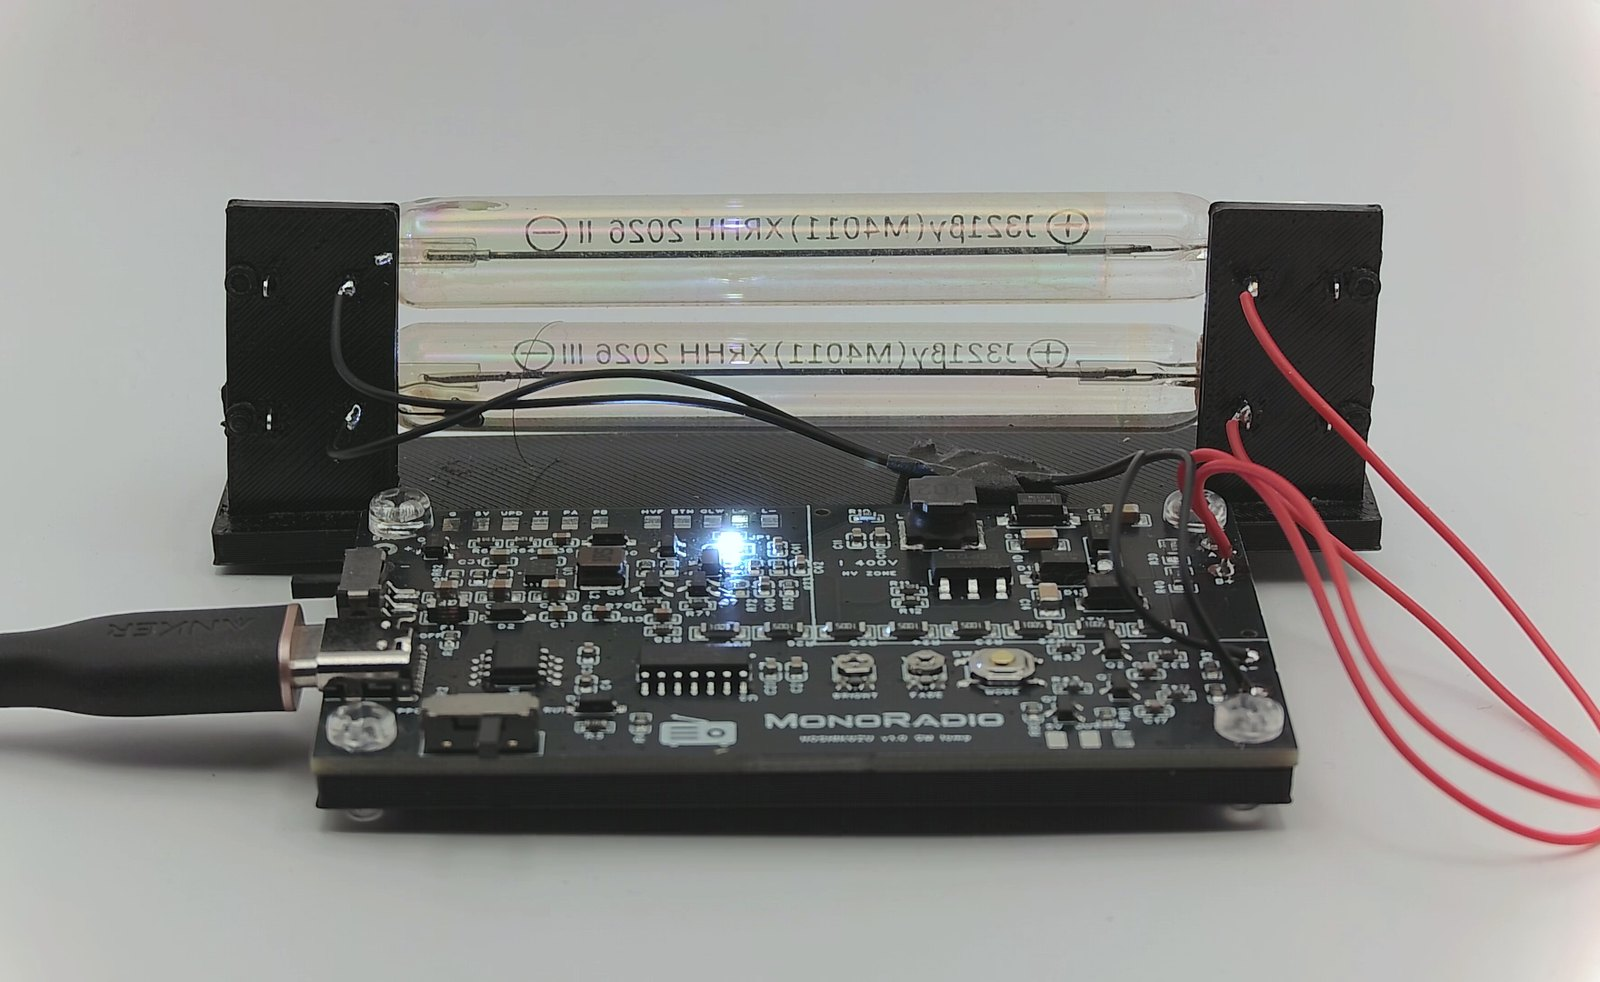
\includegraphics[width=\columnwidth]{../../../hardware/images/lamp.jpg}
\caption{Hoshikuzu-to: two stacked GM tubes (back) and the board that glows at the moment of a coincidence (front).}
\label{fig:lamp}
\end{figure}

\section{Apparatus and method}

\subsection{Detector}

The detector is a pair of J321 GM tubes lying horizontally, one above the other (Table~\ref{tab:setup}, Fig.~\ref{fig:detector}). A boost converter followed by a voltage doubler supplies the high voltage, which the microcontroller regulates at 360~V.

\begin{table}[t]
\caption{Detector and run conditions.}
\label{tab:setup}
\begin{ruledtabular}
\begin{tabular}{ll}
GM tubes & J321 $\times$ 2 (diameter 10 mm, glass 70 mm) \\
Layout & stacked, axes horizontal, $\approx$12 mm apart \\
High voltage & 360 V (run B: 359.2--360.1 V) \\
Window & $\tau = 100\us$ \\
Dead time & $\tau_d = 200\us$ per tube (firmware 1.5.0 on) \\
Site & indoors, on a desk \\
\end{tabular}
\end{ruledtabular}
\end{table}

\begin{figure*}[t]
\centering
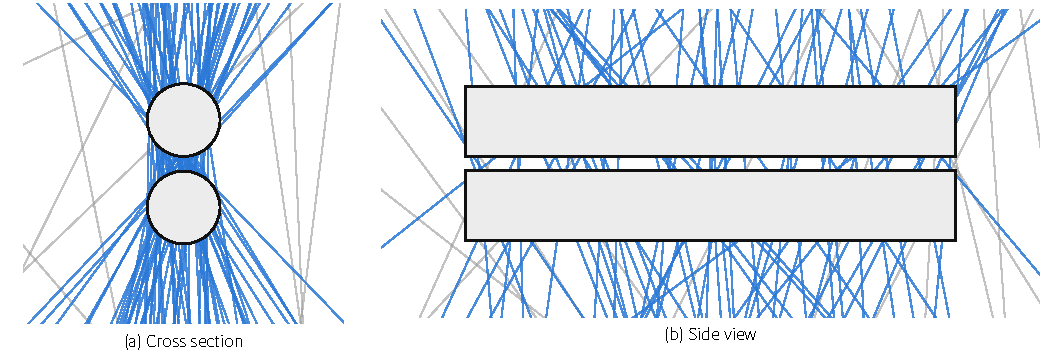
\includegraphics[width=\textwidth]{figures/en/detector.pdf}
\caption{Detector geometry. Of the lines generated in the Monte Carlo, those through both tubes (blue, counted) and others (gray).}
\label{fig:detector}
\end{figure*}

\subsection{Coincidence and counting}

The coincidence is made twice. For the light, charge flows through a two-stage PNP stack into a capacitor only while the pulses of both tubes overlap, so the window is set by the pulse overlap (about 0.1~ms). For the counts, a microcontroller (ATtiny1614) catches the falling edge of each tube's pulse in an interrupt and time-stamps it to a microsecond; a pair with $|\Delta t| \le \tau$ is a coincidence. It also counts delayed coincidences $D$ with the window shifted by 1~ms. A pulse that comes within $\tau_d = 200\us$ of the last counted pulse of the same tube is taken as a repeat of the same discharge and ignored (dead time, firmware 1.5.0 on). Counts lost to a non-paralyzable dead time are corrected by $n = m/(1 - m\tau_d)$, where $n$ and $m$ are the true and observed rates;\cite{knoll} for a single tube at 20~min$^{-1}$, $m\tau_d \approx 7\times10^{-5}$, which is negligible. All numbers in this paper come from the digital counts.

\subsection{Data taking}

The board was connected over USB to a small PC, which recorded (1)~10-s summaries (high voltage, counts of tubes A and B, coincidences $C$, delayed coincidences $D$), (2)~every hit with the PC's time stamp (ms), and (3)~for pairs within 5~ms, $\Delta t = t_B - t_A$ measured on the board ($\mu$s). Table~\ref{tab:runs} lists the two runs. The main results come from run B; run A is used in Sec.~\ref{sec:compare} to check reproducibility. Neither run has a gap longer than 25~s in its 10-s records.

\begin{table}[t]
\caption{Runs.}
\label{tab:runs}
\begin{ruledtabular}
\begin{tabular}{lccr}
 & Firmware & Start (JST) & Length \\
\hline
Run A & 1.4.0 & 2026-11-07 11:01 & 45.7 h \\
Run B & 1.6.0 & 2026-11-09 09:30 & 10.0 h \\
\end{tabular}
\end{ruledtabular}
\end{table}

\section{Results}

\subsection{Rates}

Table~\ref{tab:rates} gives the counts of run B. The single-tube counts are mostly ambient gamma rays.

\begin{table}[t]
\caption{Counts and rates (run B).}
\label{tab:rates}
\begin{ruledtabular}
\begin{tabular}{lrr}
 & Counts & Rate (min$^{-1}$) \\
\hline
Coincidences $C$ & 1,162 & $1.937 \pm 0.057$ \\
Tube A & 10,302 & 17.17 \\
Tube B & 8,130 & 13.55 \\
Delayed $D$ & 1 & --- \\
\end{tabular}
\end{ruledtabular}
\end{table}

\subsection{Arrival statistics}
\label{sec:stat}

If arrivals are independent and the rate $R$ is constant, the number $k$ counted in a time $\Delta T$ follows the Poisson distribution and the waiting time $\Delta t$ the exponential one,
\begin{gather}
P(k) = \frac{\lambda^{k} e^{-\lambda}}{k!}, \qquad \lambda = R\,\Delta T, \label{eq:poisson}\\
p(\Delta t) = R\, e^{-R\Delta t}, \qquad \Delta t_{1/2} = \frac{\ln 2}{R}. \label{eq:expo}
\end{gather}
The counts per minute have mean 1.93 and variance 1.765, as $\sigma^2 = \lambda$ requires (Fig.~\ref{fig:poisson}); a $\chi^2$ test of the whole distribution gives $\chi^2 = 9.2$ for 5 degrees of freedom ($p = 0.1$). The median waiting time, 22.3~s, matches $\Delta t_{1/2} = 21.5$~s from Eq.~\eqref{eq:expo} (Fig.~\ref{fig:intervals}), and a KS test against the exponential gives $p = 0.4$. Neither test rejects independent arrivals.

\begin{figure}[t]
\centering
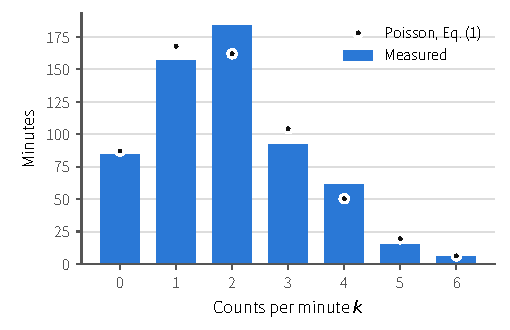
\includegraphics[width=\columnwidth]{figures/en/poisson.pdf}
\caption{Coincidences per minute (599 minutes). Dots: Eq.~\eqref{eq:poisson} with $\lambda = 1.93$.}
\label{fig:poisson}
\end{figure}

\begin{figure}[t]
\centering
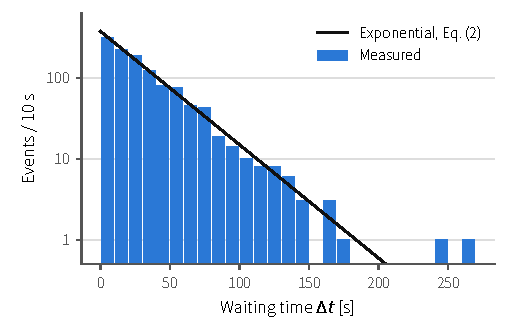
\includegraphics[width=\columnwidth]{figures/en/intervals.pdf}
\caption{Waiting times between coincidences (1,161 intervals). Line: Eq.~\eqref{eq:expo}.}
\label{fig:intervals}
\end{figure}

\subsection{Chance coincidences}

Two unrelated hits fall in the window by chance at the rate
\begin{equation}
R_\mathrm{acc} = 2\,\tau\, R_A\, R_B . \label{eq:acc}
\end{equation}
For run B this predicts 0.47 chance events inside the window, 0.04\% of the coincidences. Pairs outside the window ($0.1 < |\Delta t| \le 5$~ms) are all chance overlaps, so their distribution should be flat at the height set by Eq.~\eqref{eq:acc} (Fig.~\ref{fig:coinc}). We find 17 such pairs against 22.8 expected, and a delayed-coincidence count of 1 against 0.94 expected.

\begin{figure}[t]
\centering
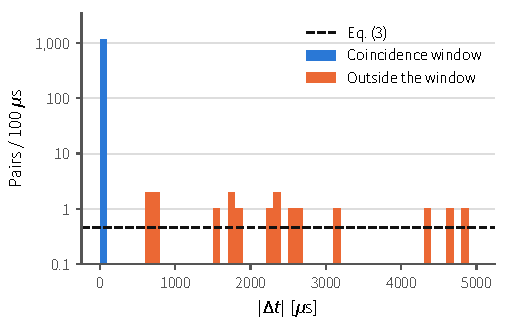
\includegraphics[width=\columnwidth]{figures/en/coincidence.pdf}
\caption{Distribution of $|\Delta t|$ between the two tubes in 100-$\mu$s bins. Dashed line: chance level from Eq.~\eqref{eq:acc}.}
\label{fig:coinc}
\end{figure}

\subsection{Time differences}

A muon crosses the two tubes, about 12~mm apart, in 0.04~ns. The measured time differences instead peak at a median of $+16\us$, with 89\% between $+9$ and $+17\us$ (Fig.~\ref{fig:dt}). This offset comes not from the flight time but from the time the microcontroller takes to service the two interrupts in turn. Both tubes share one port interrupt, and the handler services tube A first, so $\Delta t$ is shifted by the run time of A's handler (mean $+15.8\us$). When tube B falls slightly earlier, the order is reversed, which gives a small peak near $-21.4\us$ (9.5\% of all pairs).

\begin{figure}[t]
\centering
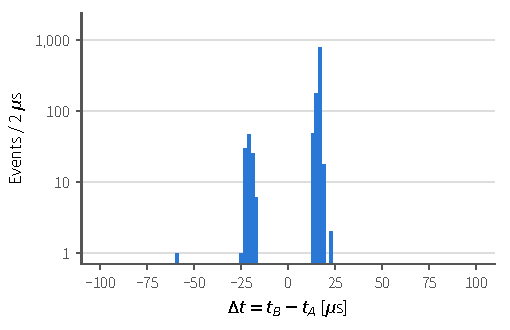
\includegraphics[width=\columnwidth]{figures/en/dt.pdf}
\caption{Time differences $\Delta t = t_B - t_A$ inside the window.}
\label{fig:dt}
\end{figure}

\subsection{Stability}

The hourly coincidence counts of run B average 116.6 with $\chi^2 = 6.3$ for 8 degrees of freedom ($p = 0.62$); run A, after correction, gives $\chi^2 = 49.9$ for 43 ($p = 0.22$). Neither shows changes beyond statistical fluctuation (Fig.~\ref{fig:hourly}).

\begin{figure*}[t]
\centering
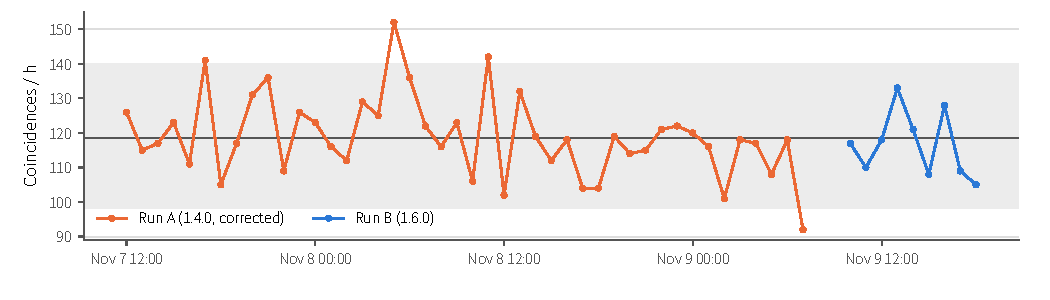
\includegraphics[width=\textwidth]{figures/en/hourly.pdf}
\caption{Hourly coincidences. The band holds 95\% of a Poisson distribution with the mean shown by the line. Run A is corrected as described in Sec.~\ref{sec:compare}.}
\label{fig:hourly}
\end{figure*}

\subsection{Comparison of the two runs}
\label{sec:compare}

Run A was taken with earlier firmware (1.4.0), before the dead time was added. Its event list contained, 6.8 times per hour, bursts of two to four coincidences within 10~ms---a pattern that independent arrivals would produce about twice in 45 hours. In each burst one tube fired again 20--96~$\mu$s after its first pulse, inside the window, so the same muon was counted again. Widening the time differences to 5~ms showed no excess of repeat pulses beyond 100~$\mu$s.

Before correction the rate of run A was 2.14~min$^{-1}$, and its hourly counts scattered more than a Poisson distribution allows ($\chi^2 = 62.5$ for 43 degrees of freedom, $p = 0.027$). Treating hits within 10~ms on the PC clock as one discharge brings the scatter back to Poisson ($\chi^2 = 49.9$, $p = 0.22$) and gives $1.98 \pm 0.03\permin$, which agrees with the $1.94 \pm 0.06\permin$ of run B within 0.7$\,\sigma$ (Table~\ref{tab:compare}). In run B the burst rate is 0.0 per hour, and repeat hits of a tube within 10~ms occur 5.1 times per hour against 4.8 expected by chance. An error that the mean alone would hide can thus be found and corrected with the same statistical tests as in Sec.~\ref{sec:stat}, provided every event is time-stamped.

\begin{table}[t]
\caption{Comparison of the two runs. $\chi^2$ is for the hourly counts; a burst is coincidences following each other within 10~ms.}
\label{tab:compare}
\begin{ruledtabular}
\begin{tabular}{lccc}
 & \multicolumn{2}{c}{Run A} & Run B \\
 & raw & corrected & \\
\hline
Rate (min$^{-1}$) & 2.14 & $1.98 \pm 0.03$ & $1.94 \pm 0.06$ \\
$\chi^2$/dof & 62.5/43 & 49.9/43 & 6.3/8 \\
Its $p$ value & 0.027 & 0.22 & 0.62 \\
Bursts (h$^{-1}$) & 6.8 & --- & 0.0 \\
\end{tabular}
\end{ruledtabular}
\end{table}

\section{Geometric acceptance and vertical intensity}

The intensity of muons at ground level depends on the zenith angle $\theta$ roughly as\cite{pdg}
\begin{equation}
I(\theta) = I_0 \cos^2\theta . \label{eq:cos2}
\end{equation}
Let $A_\perp(\theta,\phi)$ be the area, projected on a plane perpendicular to the direction $(\theta,\phi)$, of the bundle of lines that pass through both tubes. The rate is then
\begin{equation}
R = \varepsilon\, I_0\, G, \qquad G \equiv \int_\Omega \cos^2\theta\, A_\perp(\theta,\phi)\, d\Omega , \label{eq:G}
\end{equation}
where $\varepsilon$ lumps together the detection efficiency and shielding. We computed the geometric factor $G$ by a Monte Carlo that draws lines through a horizontal plane weighted by $\cos^3\theta$. Since the sensitive length of the tubes cannot be measured directly, we used both the glass length, 7~cm, and 5~cm, which leaves out the electrodes at the ends (Table~\ref{tab:geo}).

\begin{table}[t]
\caption{Geometric factor and predicted rate ($I_0 = 70\Iunit$, $\varepsilon = 1$).}
\label{tab:geo}
\begin{ruledtabular}
\begin{tabular}{ccccc}
Length & $G$ (cm$^2$\,sr) & Predicted & Measured & Ratio \\
\hline
5 cm & 4.45 & 1.87 & 1.94 & 1.04 \\
7 cm & 6.29 & 2.64 & 1.94 & 0.73 \\
\end{tabular}
\end{ruledtabular}
\end{table}

Solving Eq.~\eqref{eq:G} with $\varepsilon = 1$ gives $I_0 = R/G = 51.3$--$72.5\Iunit$. The range includes the accepted value of about $70\Iunit$.\cite{pdg} Shielding indoors and an efficiency below unity ($\varepsilon < 1$) make this consistent. The counted muons arrive at a median zenith angle of 27$^\circ$ (Fig.~\ref{fig:zenith}): the intensity peaks at the vertical, but the solid angle near the zenith is small, so the distribution peaks at 20--30$^\circ$. Systematic uncertainties in the predicted rate and in $I_0$ come from the uncertain sensitive length (the spread in Table~\ref{tab:geo}), efficiency and shielding ($\varepsilon$), and the measured tube spacing (1~mm changes $G$ by about 8\%).

\begin{figure}[t]
\centering
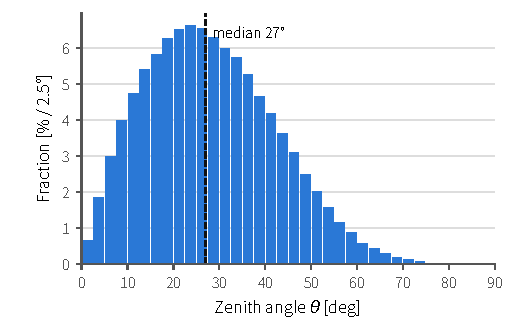
\includegraphics[width=\columnwidth]{figures/en/zenith.pdf}
\caption{Zenith angles of counted muons (Monte Carlo, 7-cm sensitive length).}
\label{fig:zenith}
\end{figure}

\section{Discussion: time dilation}

The muon lifetime is $\tau_\mu = 2.197\us$,\cite{pdg} so even at the speed of light a muon would travel only $c\tau_\mu \approx 659$~m. That muons made 15~km up are counted at the ground is due to the time dilation of special relativity,\cite{rossi,frisch}
\begin{equation}
\gamma = \frac{E}{m_\mu c^2}, \quad L = \gamma\beta c\tau_\mu, \quad \frac{N(h)}{N_0} = e^{-h/L} . \label{eq:dilation}
\end{equation}
For a typical ground-level energy $E \approx 4$~GeV, $\gamma \approx 38$ and $L \approx 25$~km, so a fraction 0.55 survives 15~km; without time dilation it would be $1.3\times 10^{-10}$ (energy loss in the air is ignored). The two coincidences a minute are a modest witness that time dilation is real.

\section{Conclusion}

A lamp built as a decorative object works as a quantitative counter of cosmic-ray muons. The coincidence rate is $1.94 \pm 0.06\permin$ and the arrivals follow a Poisson process. Chance coincidences agree with Eq.~\eqref{eq:acc} and make up 0.04\% of the total. The prediction from the tube geometry and the $\cos^2\theta$ distribution agrees with the measurement and gives $I_0 = 51.3$--$72.5\Iunit$. Statistical tests on the event record found and corrected double counting in the counting chain, and after correction the two runs agree within the errors.

\section{Further work}

The relative statistical error is $\sigma_R/R = 1/\sqrt{N}$; one lamp counts about 2,789 events a day, fixing the daily rate to $\pm1.9$\%. Tilting the pair by an angle $\alpha$ about the tube axis changes the accepted zenith angles; Fig.~\ref{fig:tilt} shows the rate ratio predicted from Eq.~\eqref{eq:G}, and a day at each angle would test Eq.~\eqref{eq:cos2}. Other studies within reach are the barometric effect ($\Delta R/R = \beta\Delta P$ with $\beta \approx -0.1$ to $-0.2$\%/hPa\cite{dorman}), Forbush decreases after solar eruptions,\cite{forbush} extensive air showers with two lamps, and the dependence on location.

\begin{figure}[t]
\centering
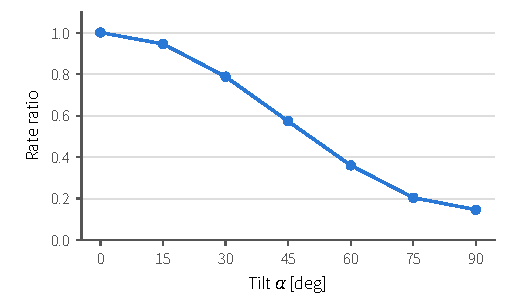
\includegraphics[width=\columnwidth]{figures/en/tilt.pdf}
\caption{Predicted rate ratio when the pair is tilted ($\alpha = 0^\circ$: stacked, $90^\circ$: side by side).}
\label{fig:tilt}
\end{figure}

\section*{Data and code}

The analysis code, results, data, schematics and firmware are available at \url{https://github.com/monoradio102/stardust-lamp}.

\begin{thebibliography}{9}
\bibitem{pdg} S.~Navas \textit{et al.} (Particle Data Group), ``Review of Particle Physics,'' Phys.\ Rev.\ D \textbf{110}, 030001 (2024).
\bibitem{rossi} B.~Rossi and D.~B.~Hall, ``Variation of the rate of decay of mesotrons with momentum,'' Phys.\ Rev.\ \textbf{59}, 223 (1941).
\bibitem{frisch} D.~H.~Frisch and J.~H.~Smith, ``Measurement of the relativistic time dilation using $\mu$-mesons,'' Am.\ J.\ Phys.\ \textbf{31}, 342 (1963).
\bibitem{knoll} G.~F.~Knoll, \textit{Radiation Detection and Measurement}, 4th ed.\ (Wiley, 2010).
\bibitem{dorman} L.~I.~Dorman, \textit{Cosmic Rays in the Earth's Atmosphere and Underground} (Springer, 2004).
\bibitem{forbush} S.~E.~Forbush, ``On the effects in cosmic-ray intensity observed during the recent magnetic storm,'' Phys.\ Rev.\ \textbf{51}, 1108 (1937).
\end{thebibliography}

\end{document}
